\section{Determining Integral Gain}

The primary reason to add integral gain to any PID controller is to reduce steady state error. 
With the exception of this critical benefit, most other effects of integral gain are undesired, such as increasing settling time and adding an additional pole to the system.
Given the lack of any systematic disturbance which could cause steady state error, 
integral gain was only added to the controller as a precaution.
Additionally, it is only enabled when the magnitude of the error signal is small (under 0.1 radians) to correct for poor PWM resolution.
Figure \ref{fig:ki} shows a typical case where the enabling threshold and gain for integration feedback is too high.

The block diagram implementing integral gain may be found in Figure \ref{fig:simulinkki}.
To prevent actions taken by the PD controller influencing the PID controller, the integrator is reset each time it is enabled. 

%Since, the PI controller is essentially a low-pass filter; the compensated system usually will have a slower rise time and longer settling time. 
%The PD controller can improve the damping and rise time of the control system at expense of higher bandwidth and resonant frequency, and the steady-state error. 
%Therefore, Integral gain is used to reduce steady state error. 
%Since, the proportional gain is very large and there is very small steady state error to begin with; the PI controller can be ignored. 
%However, it is added as contingency.

%See figures \ref{fig:ki} and \ref{fig:simulinkki}

\begin{figure}[htp]
    \centering
    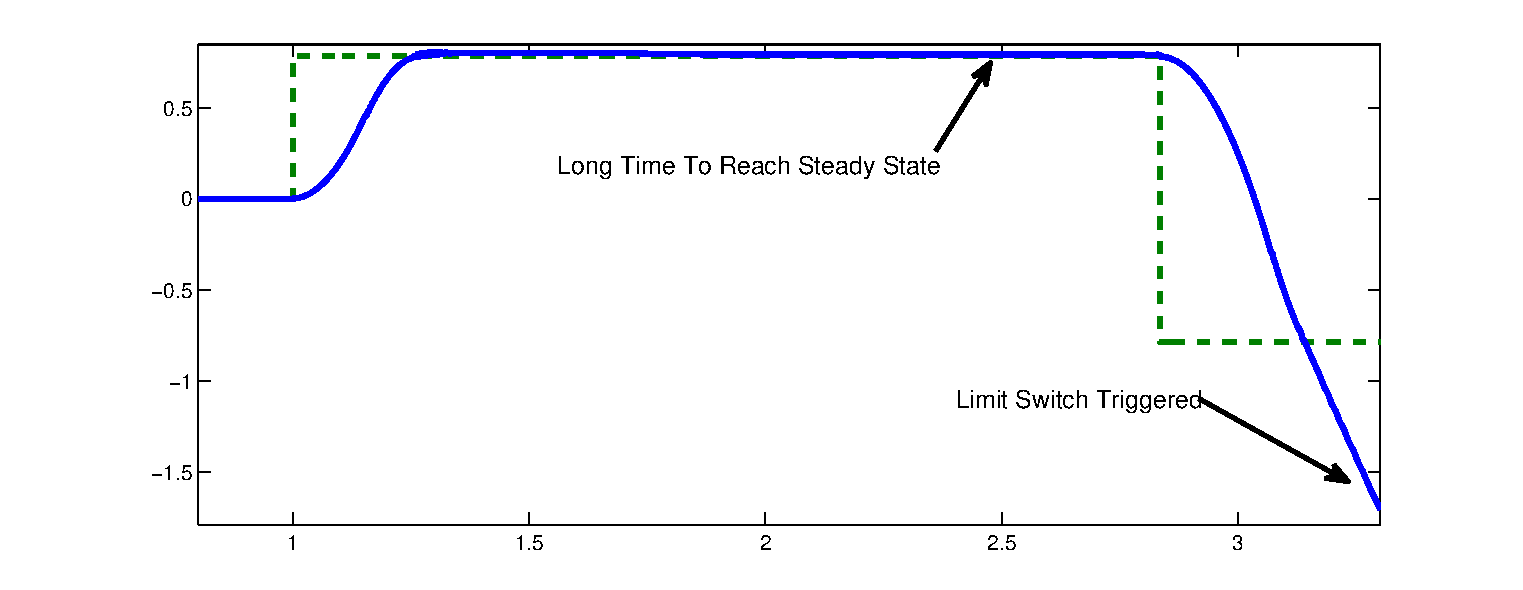
\includegraphics[width=.8\textwidth]{images/TooMuchKi.pdf}
    \caption{Too Much Integral Gain}
    \label{fig:ki}
\end{figure}

\begin{figure}[htp]
    \centering
    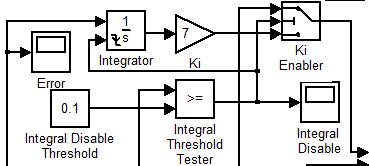
\includegraphics[scale=0.75]{images/Ki.PNG}
    \caption{Simulink Integral Gain Path}
    \label{fig:simulinkki}
\end{figure}
